\documentclass{phyasgn}
\phyasgn{
  stuname = 姚昊廷,           % 设置学生姓名
  stunum = 22322091,      % 设置学号
  setasgnnum = 1,           % 设置课程次数
  classname = 热力学和统计物理,     % 设置课程名称
}

\usepackage{listings}
\usepackage{tikz}
\usepackage{amssymb}
\usepackage{t-angles}
\usepackage{amssymb}
\usepackage{tikz}
\usepackage{mathrsfs}
\usepackage{pifont}
\usepackage{subfigure}
\usepackage{caption}
\usepackage{float}
\usepackage{mathrsfs}
%\usepackage{autobreak} 
%\usepackage{fixdif} 
\usetikzlibrary{quotes,angles}
\usetikzlibrary{calc}
\usetikzlibrary{decorations.pathreplacing}
\lstset{numbers=left,basicstyle=\ttfamily,columns=flexible}
\makeatletter
\newcommand{\rmnum}[1]{\romannumeral #1}
\newcommand{\Rmnum}[1]{\expandafter\@slowromancap\romannumeral #1@}
\renewcommand{\i}{\mathrm{i}}
\makeatother
\allowdisplaybreaks[4]%允许公式跨页
\usepackage{pdfpages}

\begin{document}

\begin{sol}[1]
    由题知
    \begin{align*}
        \mathrm{d} V&=\frac{\partial V}{\partial T}\d T+\frac{\partial V}{\partial p}\d p\\
        V&=\alpha V\d T-\kappa_T V\d p\\
    \end{align*}
    故
    \begin{align*}
        \frac{\d V}{V}&=\alpha \d T-\kappa_T \d p\\
        \ln V&=\int (\alpha\d T-\kappa_T\d p)
    \end{align*}
    代入$\alpha=\frac{1}{T},\kappa_T=\frac{1}{p}$得
    \begin{align*}
        \ln V&=\ln\frac{Tp_0}{pT_0}\\
        V&=\frac{Tp_0}{pT_0}
    \end{align*}
\end{sol}\par

\begin{sol}[2]
    \begin{align*}
        pV^n&=C\\
        npV^{n-1}\d V+V^n\d p&=0\\
        np\d V+V\d p&=0
    \end{align*}
    \begin{align*}
        pV&=\nu RT\\
        p\d V+V\d p=\nu R\d T
    \end{align*}
    联立两式,消去$V\d p$得
    \begin{align*}
        p\d V=\frac{\nu R\d T}{1-n}
    \end{align*}
    又由热力学第一定律
    \begin{align*}
        \d U&=\bar{d}Q-p\d V\\
        C_V\d T&=\bar{d}Q-p\d V\\
        \frac{\bar{d}Q}{\d T}&=C_V+\frac{\nu R}{1-n}\\
        \frac{\bar{d}Q}{\d T}&=\frac{\nu R+(1-n)C_V}{1-n}\\
        \frac{\bar{d}Q}{\d T}&=\frac{C_p-nC_V}{1-n}\\
        \frac{\bar{d}Q}{\d T}&=\frac{n-\gamma}{n-1}C_V
    \end{align*}
\end{sol}\par

\begin{sol}[3]
    选取厚度为$\d z$的一层气体进行研究,上下压力差与其所受重力抵消,故有
    \begin{align*}
        \d p=-\rho g\d z
    \end{align*}
    又绝热过程满足
    \begin{align*}
        pV^\gamma&=C\\
        \gamma pV^{\gamma-1}\d V+V^\gamma\d p&=0\\
        \gamma\frac{\d V}{V}+\frac{\d p}{p}&=0
    \end{align*}
    又
    \begin{align*}
        p V&=\nu RT\\
        V&=\frac{\nu RT}{p}\\
        \frac{\d V}{V}&=\frac{\d T}{T}-\frac{\d p}{p}
    \end{align*}
    故
    \begin{align*}
        \gamma(\frac{\d T}{T}-\frac{\d p}{p})+\frac{\d p}{p}&=0\\
        \frac{\d T}{T}&=\frac{\gamma-1}{\gamma}\frac{1}{p}\d p\\
        \frac{\d T}{\d z}&=\frac{\gamma-1}{\gamma}\frac{T}{p}\frac{\d p}{\d z}\\
        \frac{\d T}{\d z}&=\frac{\gamma-1}{\gamma}\frac{T}{p}(-\rho g)\\
    \end{align*}
    又因为
    \begin{align*}
        pV&=\nu RT\\
        pM&=\rho RT\\
        \frac{T}{p}&=\frac{M}{\rho R}
    \end{align*}
    故
    \begin{align*}
        \frac{\d T}{\d z}&=\frac{\gamma-1}{\gamma}\frac{M}{\rho R}(-\rho g)\\
        \frac{\d T}{\d z}&=\frac{1-\gamma}{\gamma}\frac{Mg}{R}
    \end{align*}
    代入$\gamma=1.4,M=29\text{g/mol},g=9.8\text{m/s}^2,R=8.31\text{J/(mol}\cdot \text{K)}$得
    \begin{align*}
        \frac{d T}{\d z}=-0.00977136K/m
    \end{align*}
\end{sol}\par

\begin{sol}[4]
    \begin{align*}
        \frac{C_p}{C_V}&=\frac{C_V+\nu R}{C_V}\\
        \gamma(T)&=1+\frac{\nu R}{C_V}
    \end{align*}
    \begin{align*}
        \d U=-p\d V\\
        C_V\d T&=-p\d V\\
        C_V\d T&=-\frac{\nu R T\d V}{V}\\
        C_V\frac{\d T}{T}&=-\frac{\nu R\d V}{V}\\
        \frac{\nu R}{\gamma-1}\frac{\d T}{T}&=-\frac{\nu R\d V}{V}\\
        \frac{1}{\gamma-1}\frac{\d T}{T}&=-\frac{\d V}{V}\\
        \ln F(T)&=-\ln V\\
        F(T)&=\frac{C}{V}
    \end{align*}
\end{sol}\par

\begin{sol}[5]
    水的熵变为
    \begin{align*}
        \Delta S_1&=\int\frac{\bar{d}Q}{T}\\
        &=\int_{273.15}^{373.15}\frac{cm\d T}{T}\\
        &=1303.99\text{J/K}
    \end{align*}
    热源熵变为
    \begin{align*}
        \Delta S_2&=\frac{Q}{T}\\
        &=\frac{-cm\Delta T}{T}\\
        &=-1120.19\text{J/K}
    \end{align*}
    故总熵变为
    \begin{align*}
        \Delta S&=\Delta S_1+\Delta S_2\\
        &=183.80\text{J/K}
    \end{align*}
    欲使$\Delta S=0$,可以使用温度在零到一百摄氏度之间的无限个热源。
\end{sol}\par

\begin{sol}[6]
    物体的熵变为
    \begin{align*}
        \Delta S_1=(S_1-S_2)
    \end{align*}
    热源的熵变为
    \begin{align*}
        \Delta S_2=\frac{Q-W}{T_2}
    \end{align*}
    由熵增原理知
    \begin{align*}
        (S_1-S_2)+\frac{Q-W}{T_2}&\geq 0\\
        W\leq Q-T_2(S_1-S_2)
    \end{align*}
    故
    \begin{align*}
        W_{max}=Q-T_2(S_1-S_2)
    \end{align*}
\end{sol}\par

\begin{sol}[7]
    \begin{figure}[H]
        \begin{tikzpicture}
            \draw[->] (0,0) --(6,0) node[right] {$S$};
            \draw[->] (0,0) --(0,6) node[above] {$T$};
            \draw[loosely dashed] (1,3) --(1,0) node[below] {$S_1$};
            \draw[loosely dashed] (4,3) --(4,0) node[below] {$S_2$};
            \draw[loosely dashed] (1,4) --(0,4) node[left] {$T_2$};
            \draw[loosely dashed] (1,3) --(0,3) node[left] {$T_1$};
            %\draw (1,3) rectangle (4,4);
            \draw[->] (1,4) --(2.5,4);
            \draw (2.5,4) --(4,4);
            \draw[->] (4,4) --(4,3.5);
            \draw (4,3.5) --(4,3);
            \draw[->] (4,3) --(2.5,3);
            \draw (2.5,3) --(1,3);
            \draw[->] (1,3) --(1,3.5);
            \draw (1,3.5) --(1,4);
        \end{tikzpicture}
    \end{figure}
    
    \begin{align*}
        W&=(S_2-S_1)(T_2-T_1)\\
        Q&=T_2(S_2-S_1)\\
        \eta&=\frac{W}{Q}=1-\frac{T_1}{T_2}
    \end{align*}
\end{sol}\par

\begin{sol}[7]
    \begin{figure}[H]
        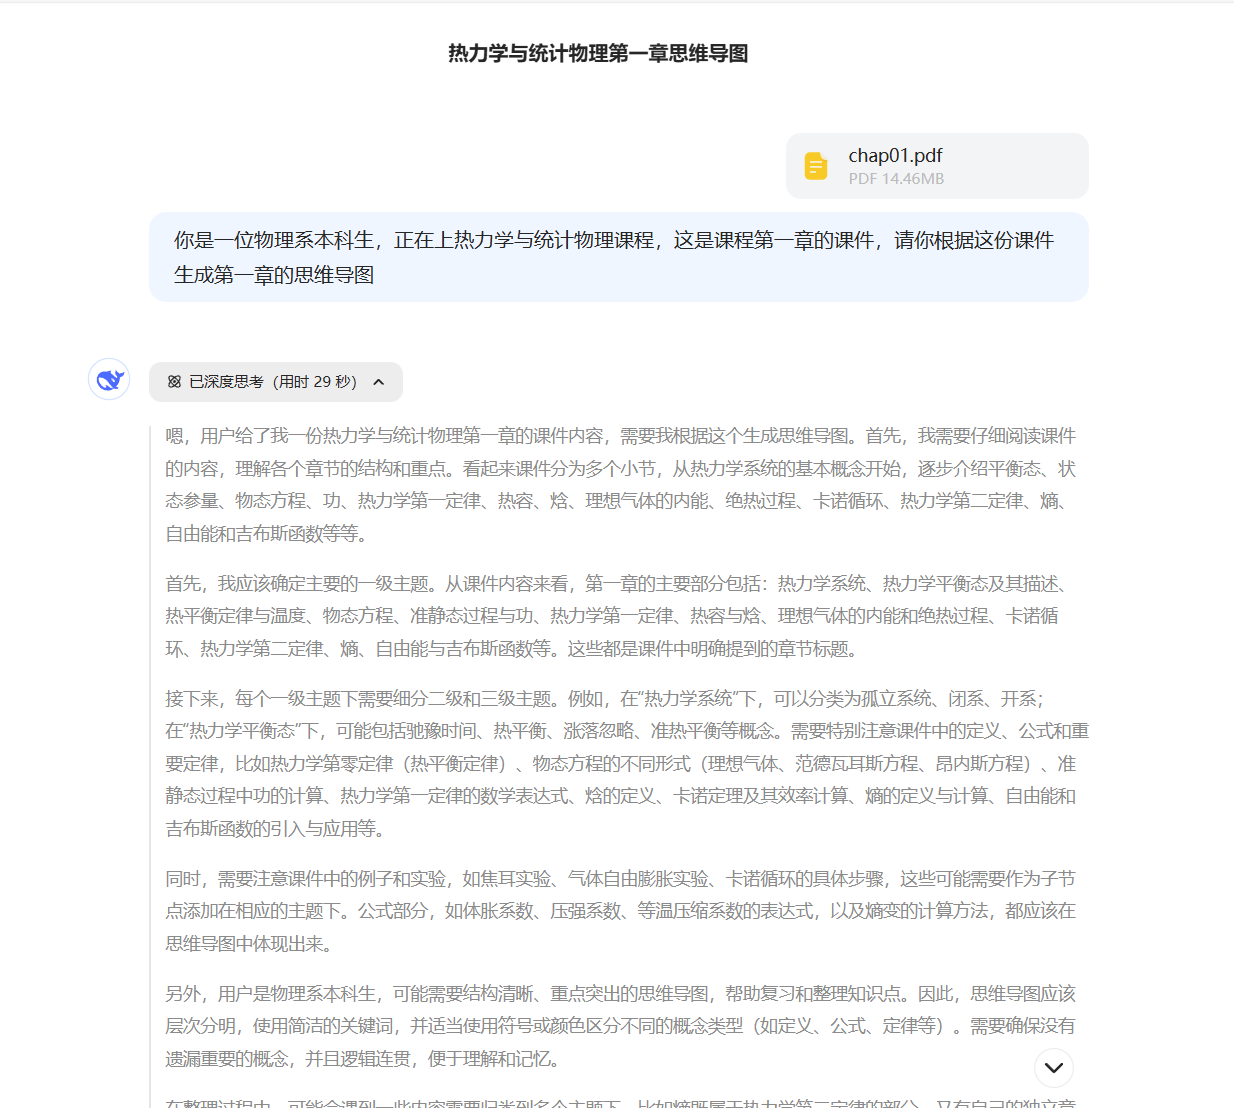
\includegraphics[width=0.5\textwidth]{企业微信截图_1742482063473.png}
    \end{figure}
    以下为ai生成
    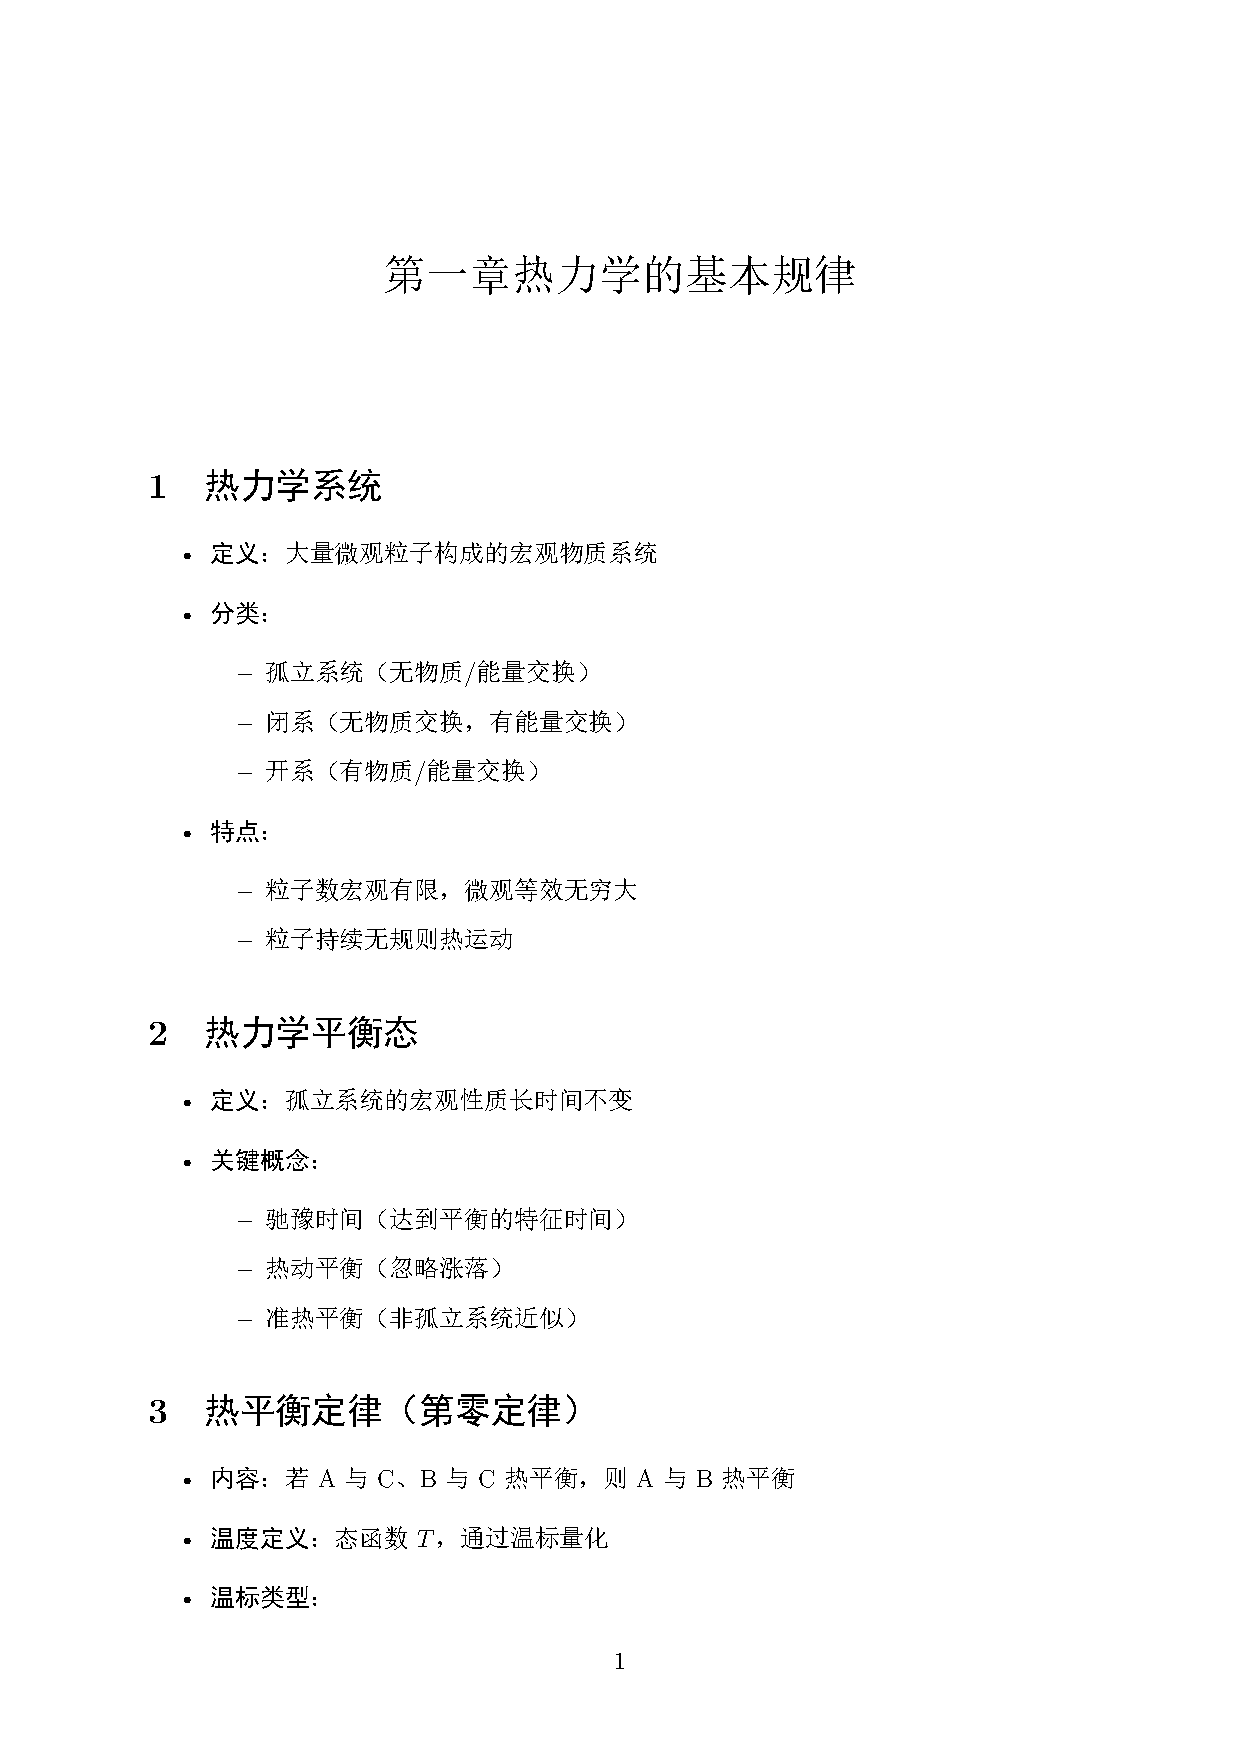
\includepdf[pages=-]{1.1.pdf}
\end{sol}\par
\end{document}